\label{cap:ingenieria}
\Needspace{.16\textheight}\section{Momento de predicción e indicadores de actividad}
El propósito de esta etapa es transformar los registros de OULAD en información que pueda utilizarse para anticipar un retiro. Para ello, primero se define a quién se observaría, hasta qué día se reuniría información y durante qué periodo posterior se buscaría el retiro.

La unidad de análisis es una inscripción: la participación de una persona en un módulo y en una edición concreta de ese módulo, denominada presentación. Una misma persona puede aportar varias inscripciones. El día 0 marca el inicio de cada edición; una fecha negativa corresponde a un momento anterior.

El día de corte, representado por $t$, es el momento al finalizar el cual se haría la predicción. Por ejemplo, en el corte 28 se reúnen los registros desde el día 0 hasta el 28, ambos incluidos: son 29 días. Ese periodo es la ventana de observación. Después del corte comienza el seguimiento, que termina al finalizar la edición del curso. La actividad anterior al día 0 se resume por separado.

Para incluir una inscripción se requiere conocer su fecha de matrícula, comprobar que ya estaba matriculada al corte y que no se había retirado hasta ese día. Además, el curso debe continuar después del corte. Por ejemplo, una inscripción retirada el día 20 no se incluye al predecir el día 28; una retirada el día 40 sí puede incluirse y tendrá un retiro futuro. Si el retiro ocurrió exactamente el día 28, también queda excluida. La Figura~\ref{editorial:temporal} ilustra estas reglas con casos hipotéticos.
\begin{figure}[htbp]\centering
\begin{tikzpicture}[x=.115cm,y=1cm,font=\small\sffamily,>=Stealth]
\fill[PUJClaro] (0,0) rectangle (28,1);
\fill[PUJResalte] (28,0) rectangle (100,1);
\node[align=center] at (14,.5) {Observación\\$[0,28]$};
\node[align=center] at (64,.5) {Seguimiento\\$(28,100]$};
\draw[->,PUJAzul] (0,0)--(104,0);
\foreach \x/\lab in {0/0,28/28,100/100}{\draw (\x,.07)--(\x,-.07) node[below]{\lab};}
\node[anchor=west] at (0,1.35) {Ejemplo hipotético: corte $t=28$ y final $L_i=100$};
\draw[dashed,gray] (28,0)--(28,-5.2);
\draw[gray] (0,-1)--(100,-1);
\fill[PUJGris] (20,-1) circle (2pt);
\node[anchor=west,fill=white] at (34,-1) {Retiro en día 20: excluida al corte};
\draw[gray] (0,-2.2)--(100,-2.2);
\fill[PUJAzul] (40,-2.2) circle (2pt);
\node[anchor=west,fill=white] at (43,-2.2) {Retiro en día 40: elegible, $Y_i=1$};
\draw[gray] (0,-3.4)--(100,-3.4);
\node[anchor=west,fill=white] at (34,-3.4) {Sin retiro registrado: elegible, $Y_i=0$};
\draw[gray] (30,-4.6)--(100,-4.6);
\draw[fill=white] (30,-4.6) circle (2pt);
\node[anchor=west,fill=white] at (34,-4.6) {Matrícula en día 30: excluida al corte};
\node[align=left,anchor=north west,text width=11.6cm] at (0,-5.4) {En los tres primeros casos, la matrícula ocurre en el día 0. Un retiro en el propio día 28 también queda excluido. La clase 0 no acredita éxito académico.};
\end{tikzpicture}
\caption{Separación entre información observada y evento futuro. Elaboración propia; casos hipotéticos, no observaciones de OULAD.}\label{editorial:temporal}
\end{figure}


Para expresar las reglas se utiliza el subíndice $i$, que identifica cada inscripción. Las fechas de matrícula, retiro y final del curso se representan con $r_i$, $u_i$ y $L_i$, respectivamente. La notación $\{0,\ldots,t\}$ incluye los días observados; $(t,L_i]$ indica que el retiro debe ocurrir después de $t$ y, como máximo, en $L_i$. La guía de la página~\pageref{editorial:notacion} reúne estos símbolos para consulta.

El conjunto $\mathcal E(t)$ contiene las inscripciones que cumplen las condiciones de inclusión. $N(t)$ cuenta esas inscripciones, $Y_i(t)$ indica si una de ellas presenta retiro futuro, $E(t)$ cuenta los retiros y $\pi(t)$ expresa su proporción:
\begin{align}
\mathcal E(t)&=\{i:r_i\text{ conocida},\ r_i\le t,\ (u_i\text{ ausente o }u_i>t),\ L_i>t\},\label{corr:elegibilidad}\\
N(t)&=|\mathcal E(t)|,\quad Y_i(t)=\mathbf 1\{t<u_i\le L_i\},\label{corr:evento}\\
E(t)&=\sum_{i\in\mathcal E(t)}Y_i(t),\qquad \pi(t)=E(t)/N(t).\label{corr:prevalencia}
\end{align}
La función $\mathbf 1$ vale uno cuando se cumple su condición y cero en otro caso; en particular, una fecha ausente no genera evento. Las barras $|\cdot|$ representan el número de elementos de un conjunto. El valor $Y_i(t)=0$, denominado clase negativa, significa que no hay un retiro registrado dentro del periodo de seguimiento. No permite afirmar que la persona haya aprobado o permanecido académicamente activa. La proporción $\pi(t)$ se calcula cuando $N(t)>0$; si no hubiera inscripciones elegibles, esa proporción no estaría definida. Los retiros del día del corte ya ocurrieron y quedan excluidos. El periodo disponible para observar un retiro se acorta cuando se predice más tarde y también depende de la duración del curso. Por eso se aplican las mismas reglas en los distintos cortes, aunque el seguimiento no dure siempre lo mismo.

Una vez seleccionadas las inscripciones, se resume su actividad. El volumen es el total de clics; la frecuencia se describe mediante los días con al menos un clic; la proporción activa indica qué parte del calendario tuvo actividad, y la intensidad indica cuántos clics hubo, en promedio, en los días activos. Para una inscripción $i$, $c_{id}$ cuenta los clics del día $d$ y $A_i(t)=\{d\in\{0,\ldots,t\}:c_{id}>0\}$ reúne los días con actividad. Con $n_t=t+1$ días observados, estas medidas se escriben como
\begin{equation}
V_i(t)=\sum_{d=0}^t c_{id},\quad k_i(t)=|A_i(t)|,\quad q_i(t)=\frac{k_i(t)}{n_t},\quad m_i(t)=\frac{V_i(t)}{k_i(t)}\quad(k_i(t)>0).\label{corr:actividad}
\end{equation}
En estas expresiones, $V_i(t)$ es el volumen, $k_i(t)$ el número de días activos, $q_i(t)$ su proporción y $m_i(t)$ la intensidad. El símbolo $\sum$ indica que se suman los clics de los días observados. La intensidad solo puede calcularse si existe al menos un día activo.

La recencia indica cuántos días han pasado desde la última interacción. Se denota $R_i(t)=t-\max A_i(t)$ donde $\max A_i(t)$ es el último día con actividad. Por ejemplo, si el corte es el día 28 y la última interacción ocurrió el 26, la recencia es de dos días. Su versión relativa divide ese tiempo por $n_t$; ambas permanecen ausentes cuando no hay actividad. El coeficiente de variación (CV) compara la dispersión de los clics con su promedio. Permite describir cuánto varía la actividad en relación con su nivel habitual. El CV de intensidad activa es la desviación estándar muestral de los clics en $A_i(t)$ dividida por su media; requiere $k_i(t)\ge2$. El CV de calendario conserva los ceros. Para abreviar, con $n=n_t$, $k=k_i(t)$ y $q=k/n$,
\begin{equation}
CV_{cal}^{2}=\frac{n}{n-1}\left[\frac{1-q}{q}+\frac{k-1}{kq}CV_{act}^{2}\right],\qquad k\ge2.\label{corr:identidadcv}
\end{equation}
Esta igualdad muestra por qué ambos CV están relacionados con la proporción de días activos. En ella, $n$ es el total de días, $k$ el número de días activos y $q$ la proporción activa. La identidad se obtiene al descomponer la suma de cuadrados de los días activos como $(k-1)s_{act}^{2}+k m^{2}$ y usar la media de calendario $qm$, donde $m$ es el promedio de clics de los días activos y $s_{act}$ su desviación estándar muestral. El primer término recoge la inactividad y el segundo la dispersión de intensidad; solo con intensidad constante se reduce a una función de $q$. Por tanto, cambiar el nombre o la definición del CV no demuestra que aporte información independiente de la frecuencia de actividad.

\paragraph{Lectura de los indicadores mediante un ejemplo}
Considérese una inscripción hipotética que cumple las condiciones para incluirse al día 28. Acumula 100 clics, tiene actividad en 10 días y su última interacción ocurrió en el día 26. El periodo incluye 29 días porque también se cuenta el día 0. La Tabla~\ref{kami:ejemploindicadores} muestra cómo se obtiene cada indicador y qué significa.
\begingroup\small\setlength{\tabcolsep}{4pt}\renewcommand{\arraystretch}{1.16}
\begin{longtable}{p{.23\linewidth}p{.24\linewidth}p{.45\linewidth}}
\caption{Lectura de los indicadores en una inscripción hipotética al día 28.}\label{kami:ejemploindicadores}\\
\toprule Indicador & Cálculo o valor & Interpretación \\\midrule\endfirsthead
\toprule Indicador & Cálculo o valor & Interpretación \\\midrule\endhead
\bottomrule\endfoot
Volumen & $V_i(28)=100$ & Se registraron 100 clics en el periodo observado.\\
Días activos & $k_i(28)=10$ & Hubo al menos un clic en 10 de los 29 días.\\
Proporción activa & $q_i(28)=10/29\simeq0{,}3448$ & Se registró actividad en aproximadamente el 34,48 por ciento de los días.\\
Intensidad & $m_i(28)=100/10=10$ & En los días activos hubo, en promedio, 10 clics.\\
Recencia & $R_i(28)=28-26=2$ & Transcurrieron dos días desde la última interacción.\\
\end{longtable}\endgroup
Estos valores resumen aspectos distintos de la participación registrada; ninguno permite, por sí solo, asignar un retiro futuro ni medir la motivación. Si no hubiera clics, el volumen y los días activos serían cero. La intensidad no podría calcularse porque no habría días activos por los cuales dividir, y la recencia tampoco, porque no existiría una última interacción observada.

La Figura~\ref{editorial:indicadores} representa el paso de registros a indicadores. La unidad resultante continúa siendo la inscripción en un corte; un conteo de filas del registro no se interpreta como número de sesiones.
\begin{figure}[htbp]\centering
\begin{tikzpicture}[font=\small\sffamily,>=Stealth,
 etapa/.style={draw=PUJAzul,text=PUJTexto,rounded corners,align=left,text width=11cm,inner sep=8pt}]
\node[etapa] (a) {\textbf{Registros de actividad disponibles hasta el corte}\\Identificación de la inscripción, fecha y clics. Las filas no identifican sesiones.};
\node[etapa,below=5mm of a] (b) {\textbf{Agregación por inscripción y día}\\Suma de clics diarios $c_{id}$ en el calendario $0,\ldots,t$; los días sin actividad aportan cero.};
\node[etapa,fill=PUJClaro,below=5mm of b] (c) {\textbf{Indicadores con interpretaciones diferentes}\\Volumen: cuánto se registra. Días activos: con qué frecuencia. Intensidad: cuánto por día activo. Recencia: cuánto tiempo desde la última actividad.};
\node[etapa,below=5mm of c] (d) {\textbf{Una fila por inscripción y corte}\\Se conservan las claves y los indicadores que no pueden calcularse. La etiqueta futura se conserva separada de los predictores.};
\draw[->,PUJAzul] (a)--(b);\draw[->,PUJAzul] (b)--(c);\draw[->,PUJAzul] (c)--(d);
\end{tikzpicture}
\caption{Transformación del registro de actividad en indicadores interpretables. Elaboración propia.}\label{editorial:indicadores}
\end{figure}


\Needspace{.25\textheight}\subsection{Lectura comparada de la variabilidad}
El CV de calendario y el CV entre días activos responden a preguntas distintas. El primero compara los clics de todos los días observados, incluidos los ceros, y combina la ausencia de actividad con la variación de su intensidad. El segundo compara únicamente los días con clics y describe cuánto varía la intensidad cuando existe actividad. Por ello, un CV activo igual a cero puede coexistir con varios días sin interacción.

La Figura~\ref{editorial:cv} presenta cuatro secuencias hipotéticas de ocho días, correspondientes al calendario inclusivo del corte 7. Todas acumulan 40 clics; los cálculos utilizan desviación estándar muestral. Esta construcción permite aislar diferencias entre indicadores sin atribuirlas a cambios de volumen ni presentarlas como observaciones del estudio.
\begin{figure}[p]\centering
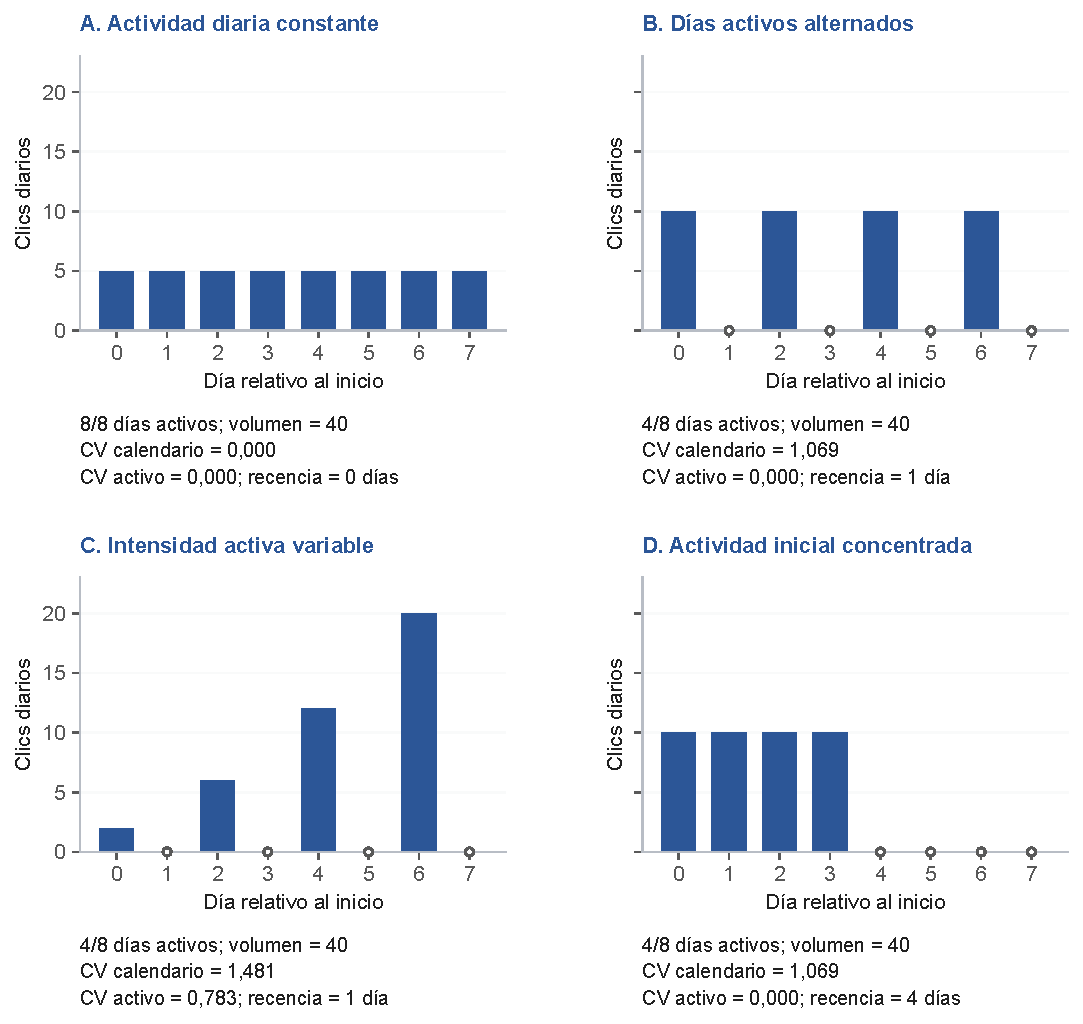
\includegraphics[width=.98\linewidth]{figuras_editoriales/comparacion_cv.pdf}
\caption{Comparación didáctica de los dos coeficientes de variación. Elaboración propia a partir de secuencias hipotéticas; los círculos sobre el eje indican días con cero clics.}\label{editorial:cv}
\end{figure}

En A se registran cinco clics todos los días y ambos CV son cero. En B se alternan días con diez clics y días sin actividad: el CV activo sigue siendo cero, pero el CV de calendario alcanza aproximadamente 1,069. Al comparar B con C se mantiene la misma cantidad de días activos; la intensidad deja de ser constante y aumentan ambos CV. Estos contrastes ilustran los dos componentes de la identidad~\eqref{corr:identidadcv}.

La comparación de B con D precisa otro límite: las secuencias contienen los mismos valores en distinto orden y, por tanto, producen los mismos CV. Sin embargo, la recencia cambia de uno a cuatro días. Los CV resumen dispersión y no identifican por sí solos el orden de la actividad; la recencia y las tendencias conservan información temporal complementaria. Ninguno de estos ejemplos establece una regla de abandono. Cuando todos los días tienen cero clics, ambos CV permanecen sin definición; cuando solo existe un día activo, no se calcula el CV activo muestral.


\Needspace{.16\textheight}\section{Criterios para seleccionar los indicadores}
\label{entrega:seleccionbase}
La selección inicial busca conservar información que describa la participación y que pueda conocerse al finalizar cada corte. Para esta versión se eligieron los clics y sus fechas, las entregas y el calendario de evaluación, y los registros de matrícula y duración de la presentación. Estas fuentes permiten construir indicadores de actividad, continuidad, inactividad, cambios temporales y participación académica. Las fechas de retiro se emplean para definir la población y el resultado futuro; no se incorporan como predictores. Los identificadores permiten unir tablas y reconocer inscripciones de una misma persona, sin tratarlos automáticamente como atributos predictivos.

La selección base de la actividad A1.3 queda documentada mediante estas inclusiones, las exclusiones explicadas a continuación y el diccionario del Anexo~\ref{corr:anexodiccionario}. El conjunto exportado contiene 26 indicadores candidatos, cotejados con su definición en el código. Los atributos sociodemográficos y de trayectoria se conservan como contexto condicionado: su inclusión en modelos requiere justificar su disponibilidad y pertinencia. Las calificaciones se mantienen únicamente para auditoría; las entregas describen participación académica y no sustituyen una medida de aprendizaje o de desempeño basada en notas.

Esta selección inicial es distinta de la selección que pueda realizarse durante el entrenamiento. Un indicador puede estar bien definido y disponible al corte sin mejorar las predicciones. Su utilidad, sus redundancias y las transformaciones necesarias deberán evaluarse dentro de los conjuntos de entrenamiento. Por tanto, documentar las variables base permite cerrar esa tarea documental en la versión actual, pero no acredita una selección predictiva final ni resuelve las ratificaciones académicas pendientes.

La variable \texttt{n\_registros\_vle} cuenta filas de actividad dentro de $[0,t]$. No cuenta sesiones, porque la fuente no permite identificarlas ni explicar todas las repeticiones. Por esta razón, se conserva para revisar los datos, pero se excluye de los candidatos del modelo. También se examinó cuánto se solapa su información con la de otros indicadores mediante el factor de inflación de la varianza (VIF), que se desarrolla en el análisis estadístico.

Los indicadores construidos no incluyen la variedad de recursos o tipos de actividad utilizados por cada inscripción. El trabajo se concentra en volumen, continuidad, recencia, cambios temporales y participación en evaluaciones, e incluye la comparación de los dos CV. Esta decisión no significa que la diversidad carezca de utilidad. Para estudiarla sería necesario integrar el catálogo de recursos y considerar que los módulos ofrecen oportunidades distintas de interacción.

El anteproyecto plantea definir el abandono a partir del retiro registrado y explorar la inactividad prolongada (actividad A3.1). También denomina voluntario a ese retiro. Los archivos permiten ubicar la baja pero no demostrar su motivo; por ello, se adopta el retiro registrado futuro y se mantiene la inactividad como indicador complementario. Por ejemplo, varios días sin clics describen una pausa en la participación, pero no confirman que la persona haya abandonado el curso. En consecuencia, la inactividad se utiliza para describir el comportamiento previo y no como un segundo resultado que el modelo deba predecir. La actividad A2.5 incluye calificaciones; estas se conservan para revisar los datos, pero no como predictores, porque se desconoce cuándo estuvieron disponibles. Estas precisiones y la selección de inscripciones que aún no se han retirado se documentan como diferencias respecto de lo previsto; su ratificación académica permanece pendiente.

Los cinco cortes representan una, dos, cuatro, seis y ocho semanas desde el inicio. Se fijaron antes de comparar modelos. Las presentaciones duran entre 234 y 269 días, por lo que el día 56 todavía está dentro del primer cuarto del curso. Esta elección permite comparar distintas cantidades de historia disponible, pero no demuestra que sean los mejores cortes posibles ni que se hayan elegido sin conocimiento previo del retiro. El calendario también permite examinar indicadores académicos, ya disponibles en el corte 14.
\Needspace{.16\textheight}\section{Población elegible y cambio de composición}
La Tabla~\ref{multi02:poblacion} responde cuántas inscripciones siguen siendo elegibles y cuántos retiros ocurren después de cada corte. Por ejemplo, al día 28 se incluyen 27\,515 inscripciones; 5\,012 tienen un retiro registrado después de ese día y hasta el final de su curso. El porcentaje es $5\,012/27\,515\times100\simeq18{,}22\,\%$. Se calcula sobre inscripciones, no sobre las 24\,826 personas distintas. La Tabla~\ref{multi02:transiciones} identifica entradas y salidas entre cortes consecutivos; por ello, la disminución del total no debe interpretarse como seguimiento de una población fija.
\Needspace{0.3\textheight}
\begingroup\small\setlength{\tabcolsep}{3pt}\renewcommand{\arraystretch}{1.16}
\begin{longtable}{>{\raggedright\arraybackslash}p{0.0870967741935484\linewidth}>{\raggedright\arraybackslash}p{0.23225806451612904\linewidth}>{\raggedright\arraybackslash}p{0.20322580645161292\linewidth}>{\raggedright\arraybackslash}p{0.22258064516129036\linewidth}>{\raggedright\arraybackslash}p{0.1548387096774194\linewidth}}
\caption{Población y evento propios de cada corte; el porcentaje usa inscripciones elegibles.}\label{multi02:poblacion}\\
\toprule
\textbf{Corte} & \textbf{Inscripciones} & \textbf{Personas} & \textbf{Retiros futuros} & \textbf{Porcentaje} \\
\midrule\endfirsthead
\toprule
\textbf{Corte} & \textbf{Inscripciones} & \textbf{Personas} & \textbf{Retiros futuros} & \textbf{Porcentaje} \\
\midrule\endhead
\bottomrule\endfoot
7 & 29\,076 & 26\,030 & 6\,632 & 22,81 \\*
14 & 28\,054 & 25\,220 & 5\,580 & 19,89 \\*
28 & 27\,515 & 24\,826 & 5\,012 & 18,22 \\*
42 & 27\,005 & 24\,491 & 4\,500 & 16,66 \\*
56 & 26\,506 & 24\,105 & 3\,998 & 15,08 \\*
\end{longtable}\endgroup
El número de inscripciones disminuye sobre todo porque se excluyen retiros que ya ocurrieron. También entran algunas matrículas nuevas entre cortes. Por tanto, las filas de la tabla no representan exactamente al mismo grupo de estudiantes. La menor proporción de retiro en los cortes posteriores no demuestra una mejora educativa: cambian el grupo analizado y el tiempo que queda para observar el evento. Las tablas de filtros y de módulo y presentación conservan los denominadores de cada comparación.

\Needspace{0.3\textheight}
\begingroup\small\setlength{\tabcolsep}{3pt}\renewcommand{\arraystretch}{1.16}
\begin{longtable}{>{\raggedright\arraybackslash}p{0.12000000000000001\linewidth}>{\raggedright\arraybackslash}p{0.12000000000000001\linewidth}>{\raggedright\arraybackslash}p{0.24000000000000002\linewidth}>{\raggedright\arraybackslash}p{0.21000000000000002\linewidth}>{\raggedright\arraybackslash}p{0.21000000000000002\linewidth}}
\caption{Cambio de composición entre cortes consecutivos.}\label{multi02:transiciones}\\
\toprule
\textbf{Desde} & \textbf{Hasta} & \textbf{Comunes} & \textbf{Salen} & \textbf{Entran} \\
\midrule\endfirsthead
\toprule
\textbf{Desde} & \textbf{Hasta} & \textbf{Comunes} & \textbf{Salen} & \textbf{Entran} \\
\midrule\endhead
\bottomrule\endfoot
7 & 14 & 28\,019 & 1\,057 & 35 \\*
14 & 28 & 27\,477 & 577 & 38 \\*
28 & 42 & 27\,001 & 514 & 4 \\*
42 & 56 & 26\,503 & 502 & 3 \\*
\end{longtable}\endgroup

\begin{figure}[htbp]\centering
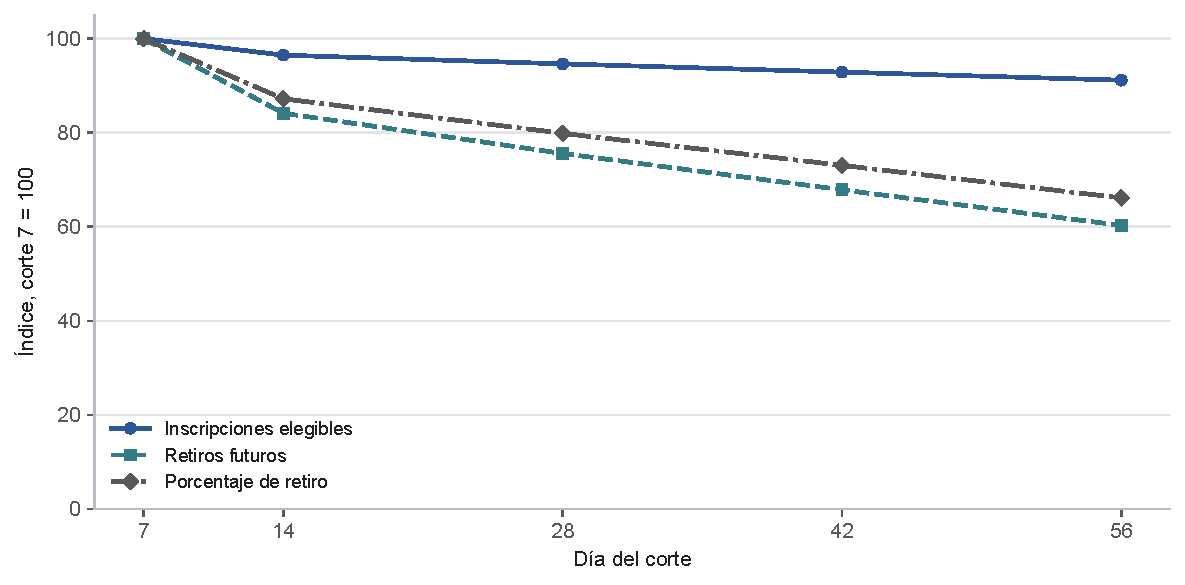
\includegraphics[width=.94\linewidth]{figuras_multiventana/02_poblacion_cortes.pdf}
\caption{Inscripciones elegibles, retiros futuros y prevalencia: índice con corte 7 igual a 100. Las líneas unen poblaciones distintas; no son trayectorias de una cohorte.}\label{multi02:figpoblacion}\end{figure}
\Needspace{.16\textheight}\section{Cascadas completas de elegibilidad}
La Figura~\ref{editorial:cascada28} resume la aplicación de los filtros al día 28. Cada exclusión se calcula sobre las inscripciones que superaron la etapa anterior, de modo que las cantidades no se suman como categorías superpuestas. El evento futuro se cuenta únicamente después de completar la elegibilidad.
\begin{figure}[htbp]\centering
\begin{tikzpicture}[font=\small\sffamily,>=Stealth,
 etapa/.style={draw=PUJAzul,text=PUJTexto,rounded corners,align=center,text width=6.2cm,minimum height=1.03cm,inner sep=5pt}]
\node[etapa] (a) at (0,0) {\textbf{Fuente completa}\\32\,593 inscripciones; 28\,785 personas};
\node[etapa] (b) at (0,-1.55) {\textbf{Fecha de matrícula conocida}\\32\,548 inscripciones; 28\,755 personas};
\node[etapa] (c) at (0,-3.1) {\textbf{Matrícula hasta el día 28}\\32\,532 inscripciones; 28\,748 personas};
\node[etapa] (d) at (0,-4.65) {\textbf{Sin retiro hasta el día 28 incluido}\\27\,515 inscripciones; 24\,826 personas};
\node[etapa,fill=PUJClaro] (e) at (0,-6.2) {\textbf{Final posterior al día 28: elegibles}\\27\,515 inscripciones; 24\,826 personas};
\draw[->,PUJAzul] (a)--(b);\draw[->,PUJAzul] (b)--(c);\draw[->,PUJAzul] (c)--(d);\draw[->,PUJAzul] (d)--(e);
\node[anchor=west,align=left,text width=4.3cm] at (3.45,-.77) {Se excluyen 45\\sin fecha de matrícula};
\node[anchor=west,align=left,text width=4.3cm] at (3.45,-2.32) {Se excluyen 16\\con matrícula posterior};
\node[anchor=west,align=left,text width=4.3cm] at (3.45,-3.87) {Se excluyen 5\,017\\con retiro hasta el corte};
\node[anchor=west,align=left,text width=4.3cm] at (3.45,-5.42) {Se excluyen 0\\por final no posterior};
\node[draw=PUJAzul,fill=PUJResalte,align=center,text width=10.4cm,inner sep=8pt] (f) at (1.7,-8) {\textbf{Evento posterior al corte, entre las elegibles}\\5\,012 retiros futuros / 27\,515 inscripciones = 18,22\,\%\\22\,503 inscripciones sin retiro registrado dentro del horizonte};
\draw[->,PUJAzul] (e.south)--(0,-7.05)--(f.north);
\end{tikzpicture}
\caption{Cascada secuencial de elegibilidad en el corte 28. Elaboración propia desde los exportables de la versión analítica del 10 de septiembre; las exclusiones cuentan inscripciones en cada etapa.}\label{editorial:cascada28}
\end{figure}

La proporción de 30,90\,\% describe fechas de retiro en la fuente completa; el 18,22\,\% utiliza 5\,012 retiros futuros entre 27\,515 inscripciones elegibles. El cambio responde a otra población y otro intervalo del evento, no a una reducción del abandono producida por el estudio. Las 5\,017 exclusiones por retiro hasta el corte coinciden numéricamente con los 5\,017 retiros posteriores al día 28 de la Tabla~\ref{rev01:retiro}; son conjuntos distintos, definidos en etapas y poblaciones diferentes.

La Tabla~\ref{corr:flujos} publica cada filtro y sus denominadores. Las exclusiones son secuenciales, no categorías superpuestas. Después del filtro de matrícula quedan 2\,643 retiros anteriores al inicio; los 35 restantes de la fuente completa ya fueron excluidos por matrícula.
\Needspace{0.2\textheight}
\begingroup\small\setlength{\tabcolsep}{3pt}\renewcommand{\arraystretch}{1.16}
\begin{longtable}{>{\raggedright\arraybackslash}p{0.0670212765957447\linewidth}>{\raggedright\arraybackslash}p{0.32553191489361705\linewidth}>{\raggedright\arraybackslash}p{0.19148936170212766\linewidth}>{\raggedright\arraybackslash}p{0.1723404255319149\linewidth}>{\raggedright\arraybackslash}p{0.14361702127659576\linewidth}}
\caption{Flujo secuencial en cada corte; las exclusiones corresponden a la etapa indicada.}\label{corr:flujos}\\
\toprule
\textbf{Corte} & \textbf{Etapa} & \textbf{Inscripciones} & \textbf{Personas} & \textbf{Excluidas} \\
\midrule\endfirsthead
\toprule
\textbf{Corte} & \textbf{Etapa} & \textbf{Inscripciones} & \textbf{Personas} & \textbf{Excluidas} \\
\midrule\endhead
\bottomrule\endfoot
7 & Fuente & 32\,593 & 28\,785 & 0 \\
7 & Matrícula conocida & 32\,548 & 28\,755 & 45 \\
7 & Matriculada al corte & 32\,455 & 28\,691 & 93 \\
7 & Sin retiro hasta corte & 29\,076 & 26\,030 & 3\,379 \\
7 & Final posterior al corte & 29\,076 & 26\,030 & 0 \\
14 & Fuente & 32\,593 & 28\,785 & 0 \\
14 & Matrícula conocida & 32\,548 & 28\,755 & 45 \\
14 & Matriculada al corte & 32\,490 & 28\,715 & 58 \\
14 & Sin retiro hasta corte & 28\,054 & 25\,220 & 4\,436 \\
14 & Final posterior al corte & 28\,054 & 25\,220 & 0 \\
28 & Fuente & 32\,593 & 28\,785 & 0 \\
28 & Matrícula conocida & 32\,548 & 28\,755 & 45 \\
28 & Matriculada al corte & 32\,532 & 28\,748 & 16 \\
28 & Sin retiro hasta corte & 27\,515 & 24\,826 & 5\,017 \\
28 & Final posterior al corte & 27\,515 & 24\,826 & 0 \\
42 & Fuente & 32\,593 & 28\,785 & 0 \\
42 & Matrícula conocida & 32\,548 & 28\,755 & 45 \\
42 & Matriculada al corte & 32\,536 & 28\,750 & 12 \\
42 & Sin retiro hasta corte & 27\,005 & 24\,491 & 5\,531 \\
42 & Final posterior al corte & 27\,005 & 24\,491 & 0 \\
56 & Fuente & 32\,593 & 28\,785 & 0 \\
56 & Matrícula conocida & 32\,548 & 28\,755 & 45 \\
56 & Matriculada al corte & 32\,539 & 28\,753 & 9 \\
56 & Sin retiro hasta corte & 26\,506 & 24\,105 & 6\,033 \\
56 & Final posterior al corte & 26\,506 & 24\,105 & 0 \\
\end{longtable}\endgroup
\Needspace{.16\textheight}\section{Construcción y disponibilidad de indicadores}
La actividad se resume mediante volumen de clics, días activos, frecuencia relativa, recencia y variabilidad de los totales diarios. Un día activo contiene al menos un clic; la proporción de días activos usa $t+1$ como denominador. Esta normalización facilita una lectura temporal, pero no corrige la menor exposición de las matrículas posteriores al inicio. Se exporta adicionalmente el número de días matriculados dentro de la ventana para identificar esta condición. El número de filas VLE no se denomina número de sesiones.

La recencia es la diferencia entre el corte y el último día activo; se conserva ausente cuando no existe actividad en la ventana. El coeficiente de variación emplea la desviación estándar muestral de los totales diarios, incluidos los ceros, dividida por su media. También se cuentan semanas completas desde el día 0 y se omite el bloque final incompleto. Estos indicadores describen conductas observables; los clics no constituyen una medición directa de motivación.

La tendencia compara bloques contiguos de igual longitud que terminan en el corte. Para $s=7$ o $s=14$, se calcula
\[
T_{i,s}(t)=\log\!\left(\frac{1+\sum_{d=t-s+1}^{t}c_{id}}
{1+\sum_{d=t-2s+1}^{t-s}c_{id}}\right).
\]
En la fórmula, $s$ es la duración de cada bloque y $T_{i,s}(t)$ es la tendencia de la inscripción $i$. El numerador suma los clics del bloque más reciente y el denominador los del anterior. Un valor positivo indica más clics recientes y uno negativo, menos. Añadir 1 permite calcular el cociente cuando uno de los bloques no tiene clics. Este suavizado conserva la inversión del signo al intercambiar los bloques, pero multiplicar todos los conteos por una misma cantidad puede cambiar el valor. Ambos bloques nulos se representan como no observables. La tendencia de siete días requiere $t\ge13$ y la de catorce $t\ge27$; 14 y 28 son los primeros cortes elegidos que cumplen esas condiciones, no los primeros matemáticamente posibles.

La inactividad acumulada y la ausencia de clics en los últimos 7, 14 o 28 días se conservan como indicadores complementarios. Una ventana reciente sin historia suficiente se representa como no observable, no como actividad ni como inactividad. Ninguno de estos indicadores binarios, con valores 0 o 1, sustituye la etiqueta administrativa; su interpretación depende del calendario y de las oportunidades de participación.

Las entregas incluyen evaluaciones distintas de \textit{Exam}, sin reconocimiento de otra presentación (\textit{banked}), observadas entre 0 y $t$. Se distinguen las evaluaciones programadas hasta el corte y cuántas de ellas ya fueron entregadas; estas últimas pueden haberse entregado antes del inicio. La proporción entregada no mide puntualidad y queda ausente cuando no hay evaluaciones programadas. Los puntajes y su disponibilidad se conservan únicamente para auditoría, porque la fecha de entrega no acredita la fecha de publicación de la nota.

\Needspace{0.3\textheight}
\begingroup\small\setlength{\tabcolsep}{3pt}\renewcommand{\arraystretch}{1.16}
\begin{longtable}{>{\raggedright\arraybackslash}p{0.07422680412371135\linewidth}>{\raggedright\arraybackslash}p{0.18556701030927839\linewidth}>{\raggedright\arraybackslash}p{0.25979381443298977\linewidth}>{\raggedright\arraybackslash}p{0.17628865979381445\linewidth}>{\raggedright\arraybackslash}p{0.2041237113402062\linewidth}}
\caption{Disponibilidad y exposición en la población elegible; conteos de inscripciones.}\label{multi02:disponibilidad}\\
\toprule
\textbf{Corte} & \textbf{Sin actividad} & \textbf{Sin evaluación programada} & \textbf{Con entregas} & \textbf{Matrícula después de 0} \\
\midrule\endfirsthead
\toprule
\textbf{Corte} & \textbf{Sin actividad} & \textbf{Sin evaluación programada} & \textbf{Con entregas} & \textbf{Matrícula después de 0} \\
\midrule\endhead
\bottomrule\endfoot
7 & 5\,316 & 29\,076 & 772 & 140 \\*
14 & 2\,551 & 26\,765 & 3\,226 & 173 \\*
28 & 1\,203 & 4\,988 & 19\,849 & 208 \\*
42 & 918 & 2\,426 & 22\,276 & 210 \\*
56 & 765 & 2\,407 & 22\,812 & 212 \\*
\end{longtable}\endgroup
En el corte 7 ninguna inscripción tiene evaluaciones con vencimiento entre 0 y 7, aunque 772 ya presentan entregas. Por ello, ausencia de entregas y falta de cumplimiento no son equivalentes. En el corte 28 persisten 4\,988 inscripciones sin evaluación programada y en el corte 56 son 2\,407; la ampliación de la ventana no elimina toda la heterogeneidad del calendario.

\Needspace{.16\textheight}\section{Disponibilidad y calendario}
La Figura~\ref{corr:calendario} muestra el primer vencimiento de evaluación según módulo y presentación, no la fecha en que cada actividad se hizo accesible. La Figura~\ref{corr:observabilidad} permite examinar qué indicadores pueden calcularse en cada corte; un porcentaje menor indica falta de observabilidad y no menor riesgo de abandono.
El primer vencimiento de evaluación continua varía entre los días 12 y 61 según la presentación. En el corte 7 hay entregas anticipadas aunque no haya vencimientos. La falta de oportunidad no equivale a incumplimiento.

\begin{figure}[H]\centering
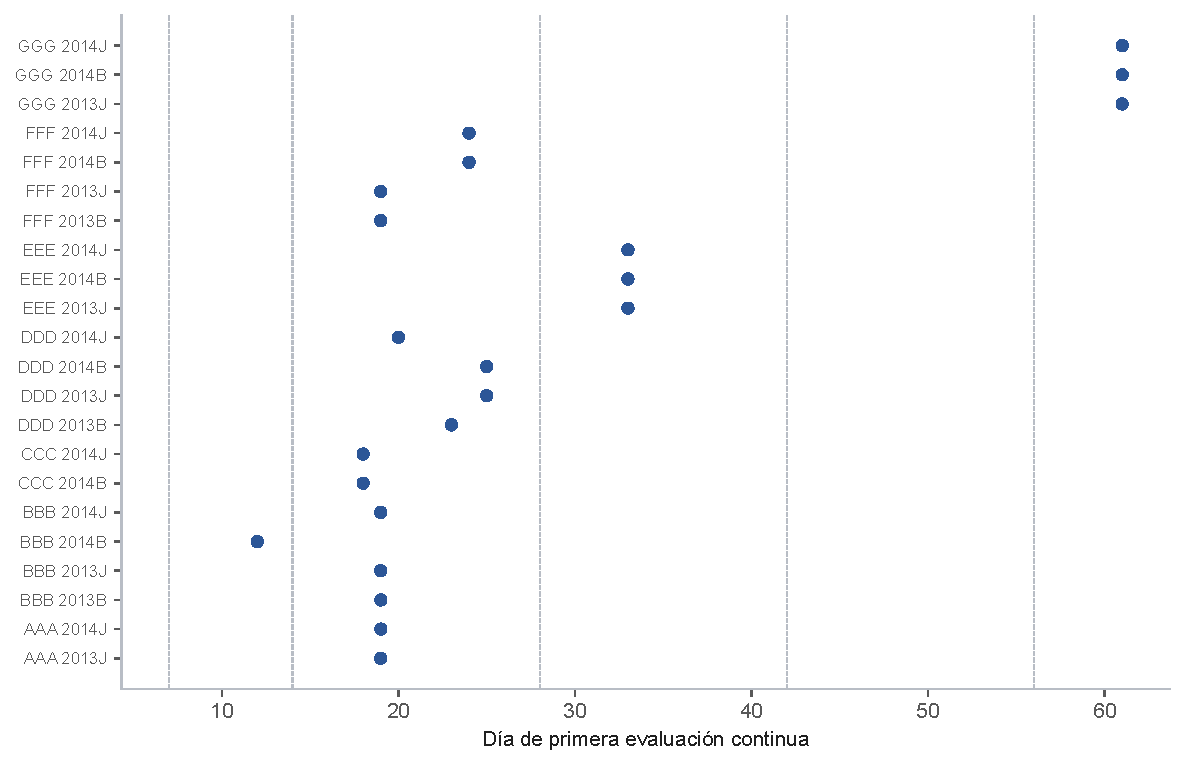
\includegraphics[width=.94\linewidth]{figuras_multiventana/02_calendario_evaluaciones.pdf}
\caption{Primer vencimiento de una evaluación distinta de examen (\textit{Exam}), por módulo y presentación.}\label{corr:calendario}\end{figure}

\begin{figure}[H]\centering
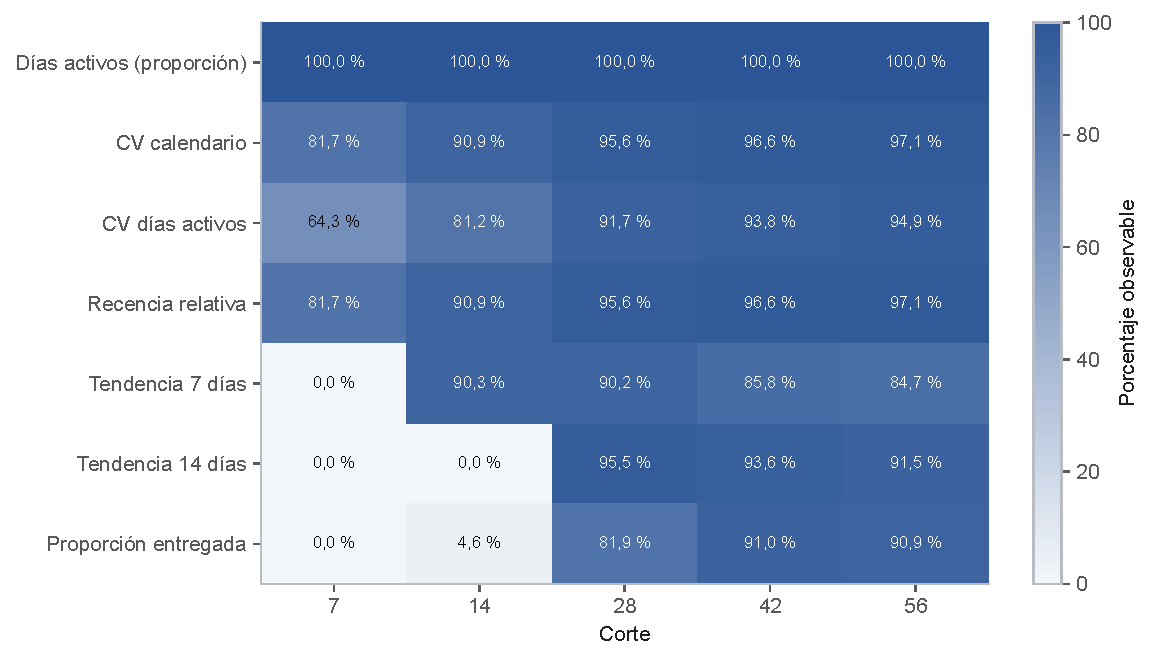
\includegraphics[width=.94\linewidth]{figuras_multiventana/02_disponibilidad_indicadores.pdf}
\caption{Disponibilidad de cada indicador para su cálculo; porcentaje de inscripciones elegibles en cada corte.}\label{corr:observabilidad}\end{figure}
Los nombres, dominios y reglas de ausencia de los candidatos se publican en el Anexo~\ref{corr:anexodiccionario}, Tabla~\ref{corr:diccionario}.
\Needspace{.16\textheight}\section{Redundancia y estructura multivariada}
Varios indicadores pueden describir aspectos cercanos de la misma actividad. Para revisar esa relación se utilizaron correlaciones, VIF y análisis de componentes principales (PCA). Las correlaciones comparan pares de variables; el VIF examina su dependencia lineal dentro de un conjunto definido; el PCA resume cómo varían en conjunto. Estos procedimientos ayudan a entender la información disponible antes del modelado.

Se calcularon correlaciones de Spearman, que comparan el orden de los valores de dos indicadores. Un signo positivo indica que valores mayores de uno tienden a acompañarse de valores mayores del otro; un signo negativo indica el orden contrario. Se contó cuántos pares de datos estaban disponibles en cada corte. El VIF se calculó con cuatro indicadores y un intercepto. El VIF indica cuánto aumenta la varianza de un coeficiente lineal por su relación con los demás predictores del conjunto. Un valor mayor señala más redundancia lineal, pero no determina qué variables serán más útiles para predecir el retiro. En particular, el volumen de clics, los días activos y las filas VLE no representan aportes completamente independientes.

El PCA combina cinco indicadores conductuales: el logaritmo de uno más los clics, la proporción de días activos, el logaritmo de uno más los clics por día activo, la recencia relativa y el CV. Se utilizan únicamente los casos con actividad y datos completos. Las variables se estandarizan restando su media y dividiendo por su desviación estándar, para llevarlas a una escala comparable y el análisis se ajusta por separado en cada corte \cite{revpca}. Cada componente es una combinación lineal de los indicadores que resume parte de su variación conjunta. El porcentaje de varianza de la Tabla~\ref{multi03:pca} expresa cuánto de esa variación recogen los dos primeros componentes. Por ello, los componentes de un corte no son los mismos ejes de los demás cortes y no deben usarse para seguir trayectorias individuales entre ventanas.

\Needspace{0.3\textheight}
\begingroup\small\setlength{\tabcolsep}{3pt}\renewcommand{\arraystretch}{1.16}
\begin{longtable}{>{\raggedright\arraybackslash}p{0.13\linewidth}>{\raggedright\arraybackslash}p{0.29\linewidth}>{\raggedright\arraybackslash}p{0.5\linewidth}}
\caption{Resumen descriptivo del PCA ajustado separadamente por corte.}\label{multi03:pca}\\
\toprule
\textbf{Corte} & \textbf{Casos observados} & \textbf{Varianza de dos componentes (\%)} \\
\midrule\endfirsthead
\toprule
\textbf{Corte} & \textbf{Casos observados} & \textbf{Varianza de dos componentes (\%)} \\
\midrule\endhead
\bottomrule\endfoot
7 & 23\,760 & 88,10 \\*
14 & 25\,503 & 87,20 \\*
28 & 26\,312 & 87,24 \\*
42 & 26\,087 & 87,57 \\*
56 & 25\,741 & 87,10 \\*
\end{longtable}\endgroup
También se utilizó el método de determinante mínimo de covarianza (MCD) para revisar observaciones alejadas del patrón conjunto de las variables. Este método estima el centro y la variación de los datos buscando reducir la influencia de valores extremos \cite{revmcd}. Se ajustó con una muestra reproducible de 5\,000 casos por corte y después se calcularon distancias para todos los casos completos. Se marcaron los que superaron el percentil empírico 97,5 de esas distancias. La marca es descriptiva: no equivale a una probabilidad de anomalía ni a una prueba de Hotelling, y no se eliminaron observaciones. Los resultados detallados de MCD, PCA y VIF se conservan en los CSV.

\Needspace{.16\textheight}\section{VIF publicado y decisión sobre el conteo de filas}
La Tabla~\ref{corr:vif} conserva la especificación utilizada para auditar la redundancia del conteo de filas. Su publicación permite justificar la decisión de exclusión sin presentar ese conjunto de cuatro variables como el diseño definitivo del clasificador.
\Needspace{0.3\textheight}
\begingroup\small\setlength{\tabcolsep}{3pt}\renewcommand{\arraystretch}{1.16}
\begin{longtable}{>{\raggedright\arraybackslash}p{0.08617021276595743\linewidth}>{\raggedright\arraybackslash}p{0.17234042553191486\linewidth}>{\raggedright\arraybackslash}p{0.15319148936170213\linewidth}>{\raggedright\arraybackslash}p{0.18191489361702126\linewidth}>{\raggedright\arraybackslash}p{0.15319148936170213\linewidth}>{\raggedright\arraybackslash}p{0.15319148936170213\linewidth}}
\caption{VIF con intercepto en la especificación de auditoría de cuatro indicadores.}\label{corr:vif}\\
\toprule
\textbf{Corte} & \textbf{n} & \textbf{Clics} & \textbf{Proporción activa} & \textbf{Filas VLE} & \textbf{Entregas} \\
\midrule\endfirsthead
\toprule
\textbf{Corte} & \textbf{n} & \textbf{Clics} & \textbf{Proporción activa} & \textbf{Filas VLE} & \textbf{Entregas} \\
\midrule\endhead
\bottomrule\endfoot
7 & 29\,076 & 3,707 & 3,388 & 6,656 & 1,052 \\*
14 & 28\,054 & 4,452 & 4,045 & 8,495 & 1,049 \\*
28 & 27\,515 & 5,235 & 4,696 & 10,929 & 1,319 \\*
42 & 27\,005 & 5,839 & 5,372 & 12,334 & 1,323 \\*
56 & 26\,506 & 6,157 & 5,673 & 13,694 & 1,394 \\*
\end{longtable}\endgroup
El mayor VIF corresponde al conteo de filas en cada corte y llega a 10,929 al día 28. Se conserva esta especificación como diagnóstico de la decisión de exclusión; no es el conjunto predictivo final. La redundancia y la procedencia no resuelta del conteo se consideran conjuntamente, sin imponer un umbral universal para todos los modelos.
\Needspace{.16\textheight}\section{Sensibilidad de variabilidad y componentes principales}
La Tabla~\ref{corr:cv} contrasta los dos CV con la proporción de días activos. Las dos columnas de observabilidad informan tamaños distintos, pero ambas correlaciones se calcularon sobre los mismos casos con al menos dos días activos. Esta precisión evita comparar correlaciones como si procedieran de las dos poblaciones observables completas.
\Needspace{0.3\textheight}
\begingroup\small\setlength{\tabcolsep}{3pt}\renewcommand{\arraystretch}{1.16}
\begin{longtable}{>{\raggedright\arraybackslash}p{0.09574468085106384\linewidth}>{\raggedright\arraybackslash}p{0.2297872340425532\linewidth}>{\raggedright\arraybackslash}p{0.22021276595744685\linewidth}>{\raggedright\arraybackslash}p{0.1819148936170213\linewidth}>{\raggedright\arraybackslash}p{0.17234042553191492\linewidth}}
\caption{Correlación con proporción activa en los mismos casos con al menos dos días activos.}\label{corr:cv}\\
\toprule
\textbf{Corte} & \textbf{CV calendario observable} & \textbf{CV activo observable} & \textbf{Rho calendario} & \textbf{Rho activo} \\
\midrule\endfirsthead
\toprule
\textbf{Corte} & \textbf{CV calendario observable} & \textbf{CV activo observable} & \textbf{Rho calendario} & \textbf{Rho activo} \\
\midrule\endhead
\bottomrule\endfoot
7 & 23\,760 & 18\,704 & -0,848 & 0,126 \\*
14 & 25\,503 & 22\,779 & -0,892 & 0,153 \\*
28 & 26\,312 & 25\,227 & -0,909 & 0,102 \\*
42 & 26\,087 & 25\,323 & -0,918 & 0,102 \\*
56 & 25\,741 & 25\,147 & -0,926 & 0,076 \\*
\end{longtable}\endgroup
La asociación con la proporción activa es menor en valor absoluto para el CV activo que para el CV de calendario en todos los cortes de la Tabla~\ref{corr:cv}. Esta diferencia es compatible con sus definiciones, ilustradas en la Figura~\ref{editorial:cv}, y se obtiene a costa de una menor observabilidad. No se identifica independencia estadística ni ganancia predictiva. El CV de calendario combina ambos componentes y no se descarta retrospectivamente como cálculo erróneo.
La Figura~\ref{fig:cv-actividad} facilita esta comparación: el CV de calendario presenta una relación negativa más marcada con la proporción de días activos, mientras el CV entre días activos muestra valores positivos próximos a cero. En cada corte, ambas series utilizan las mismas inscripciones con al menos dos días activos. Las líneas conectan resúmenes de cortes distintos; no representan trayectorias individuales ni un contraste de cambios en el tiempo.
\begin{figure}[H]\centering
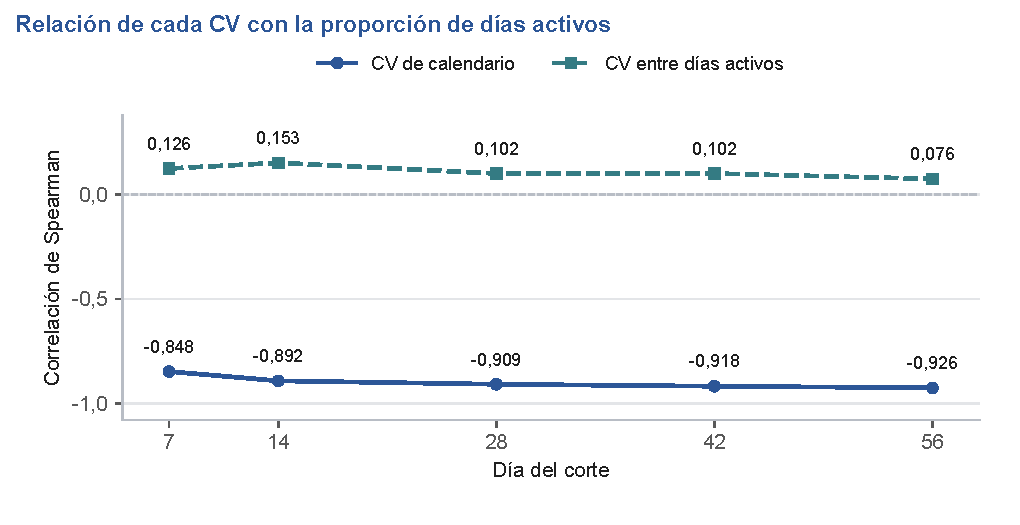
\includegraphics[width=\linewidth]{figuras_contexto/relacion_cv_actividad.pdf}
\caption[Relación entre variabilidad de clics y proporción de días activos.]{Relación entre variabilidad de clics y proporción de días activos. Elaboración propia a partir de las dos correlaciones sobre casos comunes de la Tabla~\ref{corr:cv}; se conservan en ella los conteos de observabilidad.}\label{fig:cv-actividad}
\end{figure}
En los cortes 7 y 14, los intervalos puntuales del efecto biserial del CV activo frente al retiro futuro incluyen cero y no respaldan una dirección clara. Esta diferencia respecto del CV de calendario muestra que cambiar la definición modifica la interpretación del indicador; no prueba ausencia de utilidad conjunta en un clasificador.
\Needspace{0.3\textheight}
\begingroup\small\setlength{\tabcolsep}{3pt}\renewcommand{\arraystretch}{1.16}
\begin{longtable}{>{\raggedright\arraybackslash}p{0.09574468085106384\linewidth}>{\raggedright\arraybackslash}p{0.1819148936170213\linewidth}>{\raggedright\arraybackslash}p{0.22021276595744685\linewidth}>{\raggedright\arraybackslash}p{0.22021276595744685\linewidth}>{\raggedright\arraybackslash}p{0.1819148936170213\linewidth}}
\caption{Varianza porcentual de dos componentes; comparación descriptiva sobre la misma población.}\label{corr:pcasens}\\
\toprule
\textbf{Corte} & \textbf{n común} & \textbf{Original (5)} & \textbf{Sin volumen (4)} & \textbf{CV activo (4)} \\
\midrule\endfirsthead
\toprule
\textbf{Corte} & \textbf{n común} & \textbf{Original (5)} & \textbf{Sin volumen (4)} & \textbf{CV activo (4)} \\
\midrule\endhead
\bottomrule\endfoot
7 & 18\,704 & 84,27 & 80,53 & 68,57 \\*
14 & 22\,779 & 84,73 & 81,25 & 69,00 \\*
28 & 25\,227 & 85,95 & 82,91 & 70,48 \\*
42 & 25\,323 & 86,61 & 83,72 & 70,76 \\*
56 & 25\,147 & 86,34 & 83,41 & 69,77 \\*
\end{longtable}\endgroup
La primera versión del PCA utiliza los cinco indicadores originales. La segunda retira el volumen de clics. La tercera, además, reemplaza el CV de calendario por el CV entre días activos. Las tres versiones se ajustan sobre los mismos casos, con variables estandarizadas y por separado en cada corte. Como cambia el conjunto de variables, también cambia la variación que se intenta resumir. Un porcentaje mayor no significa que el PCA explique mejor el abandono.
\Needspace{.16\textheight}\section{Sensibilidad de asociaciones a los duplicados exactos}
La Tabla~\ref{corr:duplicadosefectos} muestra cuánto cambia cada asociación al retirar filas exactamente repetidas antes de agregar la actividad. La diferencia se calcula restando el efecto de la fuente original al de la alternativa sin duplicados exactos; un valor próximo a cero indica un cambio descriptivo pequeño en esa comparación, no la validación de una política general de deduplicación.
\Needspace{0.42\textheight}
\begingroup\small\setlength{\tabcolsep}{3pt}\renewcommand{\arraystretch}{1.16}
\begin{longtable}{>{\raggedright\arraybackslash}p{0.2709677419354839\linewidth}>{\raggedright\arraybackslash}p{0.12580645161290321\linewidth}>{\raggedright\arraybackslash}p{0.12580645161290321\linewidth}>{\raggedright\arraybackslash}p{0.12580645161290321\linewidth}>{\raggedright\arraybackslash}p{0.12580645161290321\linewidth}>{\raggedright\arraybackslash}p{0.12580645161290321\linewidth}}
\caption{Cambio del efecto biserial al retirar duplicados exactos: alternativa menos fuente original.}\label{corr:duplicadosefectos}\\
\toprule
\textbf{Indicador} & \textbf{7} & \textbf{14} & \textbf{28} & \textbf{42} & \textbf{56} \\
\midrule\endfirsthead
\toprule
\textbf{Indicador} & \textbf{7} & \textbf{14} & \textbf{28} & \textbf{42} & \textbf{56} \\
\midrule\endhead
\bottomrule\endfoot
CV calendario & -0,0007 & -0,0001 & 0,0005 & 0,0003 & 0,0009 \\*
CV activo & -0,0024 & -0,0013 & -0,0004 & -0,0003 & 0,0007 \\*
Tendencia 14 & No aplica & No aplica & -0,0002 & 0,0013 & 0,0004 \\*
Tendencia 7 & No aplica & 0,0011 & 0,0005 & 0,0000 & 0,0008 \\*
Proporción activa & 0,0000 & 0,0000 & 0,0000 & 0,0000 & 0,0000 \\*
Recencia & 0,0000 & 0,0000 & 0,0000 & 0,0000 & 0,0000 \\*
Clics & 0,0001 & 0,0007 & 0,0007 & 0,0011 & 0,0014 \\*
\end{longtable}\endgroup
La alternativa elimina repeticiones en todas las columnas de la fuente antes de agregar; conserva población y evento. La actividad original sigue siendo el análisis principal. Estas diferencias cuantifican sensibilidad descriptiva, no identifican cuál registro es verdadero ni prueban robustez de un modelo aún no entrenado.
\Needspace{.16\textheight}\section{Estabilidad de los intervalos por remuestreo}
La Tabla~\ref{corr:bootstrap} examina cuánto cambian los extremos de los intervalos al ampliar el número de remuestreos. Las 66 comparaciones publicadas permanecen dentro de la tolerancia descriptiva de 0,005; este resultado caracteriza la secuencia utilizada y no una garantía general de convergencia.
\Needspace{0.3\textheight}
\begingroup\small\setlength{\tabcolsep}{3pt}\renewcommand{\arraystretch}{1.16}
\begin{longtable}{>{\raggedright\arraybackslash}p{0.14\linewidth}>{\raggedright\arraybackslash}p{0.25\linewidth}>{\raggedright\arraybackslash}p{0.29\linewidth}>{\raggedright\arraybackslash}p{0.26\linewidth}}
\caption{Cambio máximo de extremos entre 2.000 y 5.000 remuestreos; comparación numérica, no contraste de hipótesis.}\label{corr:bootstrap}\\
\toprule
\textbf{Corte} & \textbf{Indicadores} & \textbf{Cambio máximo} & \textbf{Dentro de 0,005} \\
\midrule\endfirsthead
\toprule
\textbf{Corte} & \textbf{Indicadores} & \textbf{Cambio máximo} & \textbf{Dentro de 0,005} \\
\midrule\endhead
\bottomrule\endfoot
7 & 11 & 0,0006 & 11 \\*
14 & 13 & 0,0030 & 13 \\*
28 & 14 & 0,0009 & 14 \\*
42 & 14 & 0,0008 & 14 \\*
56 & 14 & 0,0013 & 14 \\*
\end{longtable}\endgroup
Se compararon los resultados obtenidos con las primeras 500 y 2\,000 repeticiones con los de las 5\,000 de una misma secuencia. Se tomó como referencia una diferencia de 0,005 unidades del efecto entre extremos de los intervalos. Al compartir repeticiones, esta comprobación muestra estabilidad numérica en la secuencia utilizada, pero no asegura el mismo resultado con otras semillas. Los intervalos publicados utilizan 5\,000 remuestreos y mantienen su carácter exploratorio.

\Needspace{.16\textheight}\section{Sensibilidad con población y evento comunes}
Para examinar cuánto influyen los cambios de población, se repitió la comparación con las 26\,429 inscripciones que seguían siendo elegibles en los cinco cortes. En este grupo se definió un mismo evento: retiro después del día 56 y hasta el final de la presentación, con 3\,985 casos. Se compararon cinco indicadores en cada corte. Aunque el grupo y el evento se mantienen, algunos indicadores solo pueden calcularse cuando hay actividad o evaluaciones programadas, por lo que sus tamaños observados todavía pueden variar.

\Needspace{0.3\textheight}
\begingroup\small\setlength{\tabcolsep}{3pt}\renewcommand{\arraystretch}{1.16}
\begin{longtable}{>{\raggedright\arraybackslash}p{0.3375\linewidth}>{\raggedright\arraybackslash}p{0.1125\linewidth}>{\raggedright\arraybackslash}p{0.1125\linewidth}>{\raggedright\arraybackslash}p{0.1125\linewidth}>{\raggedright\arraybackslash}p{0.1125\linewidth}>{\raggedright\arraybackslash}p{0.1125\linewidth}}
\caption{Efectos descriptivos en la cohorte común, sin intervalos ni contraste entre cortes.}\label{multi03:comun}\\
\toprule
\textbf{Indicador} & \textbf{7} & \textbf{14} & \textbf{28} & \textbf{42} & \textbf{56} \\
\midrule\endfirsthead
\toprule
\textbf{Indicador} & \textbf{7} & \textbf{14} & \textbf{28} & \textbf{42} & \textbf{56} \\
\midrule\endhead
\bottomrule\endfoot
CV de calendario & 0,067 & 0,082 & 0,103 & 0,114 & 0,140 \\*
CV entre días activos & -0,011 & 0,000 & 0,040 & 0,044 & 0,046 \\*
Tendencia de 7 días & No aplica & -0,010 & -0,042 & -0,074 & 0,013 \\*
Proporción de días activos & -0,074 & -0,087 & -0,089 & -0,102 & -0,128 \\*
Proporción programada entregada & No aplica & -0,097 & -0,101 & -0,118 & -0,199 \\*
\end{longtable}\endgroup
Este grupo solo puede formarse después de saber quiénes siguen siendo elegibles en el día 56. Por eso sirve para revisar los resultados, pero no para definir a quién se alertaría en el día 7: en ese momento aún no se dispone de esa información. La comparación ayuda a reconocer que el cambio de población importa; no permite medir por sí sola cuánto del cambio se debe a la duración de la ventana.

\Needspace{.16\textheight}\section{Conclusiones y continuidad}
La comparación documenta que la disponibilidad académica y el significado de los indicadores cambian con el momento de observación. Las señales conductuales conservan asociaciones descriptivas con el retiro, mientras que algunas tendencias recientes presentan resultados menos definidos. La evidencia favorece mantener explícitos los denominadores, el calendario y la historia requerida, en lugar de completar automáticamente con ceros los indicadores no observables.

Los resultados dejan preparados los datos para comparar modelos, pero aún no señalan la mejor ventana. Esa elección deberá considerar qué tan bien se distinguen los retiros, si las probabilidades estimadas se ajustan a lo observado y cuánto tiempo queda para actuar. Las reglas de comparación deben fijarse antes de seleccionar modelos, cortes o umbrales. Además, ya se exploró la fuente completa: separar ahora un conjunto y llamarlo prueba final no permite afirmar que nunca se utilizó información de él.
